\PassOptionsToPackage{svgnames}{xcolor}
\documentclass[12pt]{article}



\usepackage[margin=1in]{geometry}  
\usepackage{graphicx}             
\usepackage{amsmath}              
\usepackage{amsfonts}              
\usepackage{framed}               
\usepackage{amssymb} 
\usepackage{array}
\usepackage{amsthm}
\usepackage[nottoc]{tocbibind}
\usepackage{bm}
\usepackage{enumitem}


  \newcommand\norm[1]{\left\lVert#1\right\rVert}
\setlength{\parindent}{0cm}
\setlength{\parskip}{0em}
\newcommand{\Lim}[1]{\raisebox{0.5ex}{\scalebox{0.8}{$\displaystyle \lim_{#1}\;$}}}
\newtheorem{definition}{Definition}[section]
\newtheorem{theorem}{Theorem}[section]
\newtheorem{notation}{Notation}[section]
\theoremstyle{definition}
\DeclareMathOperator{\arcsec}{arcsec}
\DeclareMathOperator{\arccot}{arccot}
\DeclareMathOperator{\arccsc}{arccsc}
\DeclareMathOperator{\PV}{PV}
\DeclareMathOperator{\TV}{TV}
\DeclareMathOperator{\diff}{d}
\DeclareMathOperator{\expec}{E}
\DeclareMathOperator{\var}{Var}
\DeclareMathOperator{\cov}{Cov}
\DeclareMathOperator{\CE}{CE}
\DeclareMathOperator{\RP}{RP}
\newcommand\cf[1]{\mathbf{#1}}
\setcounter{tocdepth}{1}
\setcounter{section}{-1}
\begin{document}

\title{Revision notes - MA3269}
\author{Ma Hongqiang}
\maketitle
\tableofcontents

\clearpage
%\twocolumn
\section{Preliminary Result}
\subsection{Summation of series}
\begin{itemize}
  \item $\sum_{i=0}^n y^i = \frac{1-y^{n+1}}{1-y}$
  \item $\sum_{i=0}^\infty y^i = \frac{1}{1-y}\text{ provided }|r|<1$.
  \item $\sum_{i=1}^n iy^{i-1} = \frac{1-y^n(1+n-ny)}{(1-y)^2}$
  \item $\sum_{i=1}^\infty iy^{i-1} = \frac{1}{(1-y)^2}\text{ provided }|r|<1$.
  \item $\sum_{i=1}^n iy^{i} = \frac{y(1-y^n)-ny^{n+1}(1-y)}{(1-y)^2}$
  \item $\sum_{i=1}^\infty iy^{i} = \frac{y}{(1-y)^2}\text{ provided }|r|<1$.  
  \item $\sum_{i=1}^n i = \frac{1}{2}n(n+1)$
  \item $\sum_{i=1}^n i^2 = \frac{1}{6}n(n+1)(2n+1)$
  \item $\sum_{i=1}^n i^3 = \frac{1}{4}n^2(n+1)^2$
\end{itemize}
\subsection{Newton Rhapson Method}
\[
x_{i+1} = x_i-\frac{f(x_i)}{f^\prime(x_i)}
\]
\subsection{Force of Interest}
Accumulation function $a(s,t)$ can be derived from \textbf{force of interest} as such:
\[
a(s,t) = e^{\int_s^t \delta(r)\diff r}
\]
where $\delta(r)$ is the force of interest with $s\leq r\leq t$.
\subsection{Standard Derivatives}

\clearpage
\section{Theory of Interest}
\subsection{Interest}
\begin{definition}[Accumulation Function]
\hfill\\\normalfont When a principal of 1 dollar is deposited in an interest-paying account at time $t=0$, it earns some interest over the time interval $[0,t]$. \\
The accumulated value of 1 dollar at time $t \geq 0$, denoted by $a(t)$, is known as the \textbf{accumulation function}. Clearly, $a(0)=1$.
\end{definition}
\begin{definition}[Simple and Compound Interest]
\hfill\\\normalfont Let $r$ be the annual rate of interest.\\
Based on the \textbf{simple-interest} method of calculating interest,
\[
a(t)=1+rt\;\;\;\text{for }t \geq 0
\]
If the \textbf{compound interest} method is used,
\[
a(t)=(1+r)^t \;\;\;\text{for }t\geq 0
\]
\end{definition}
Suppose the interest rate is $r_i$ for the period $[\sum_{k=0}^{i-1} t_i,\sum_{k=1}^{i} t_{i} ]$, where $t_0 = 0$, 
\[
a(t_j)=1+\sum_{i=1}^j r_it_i \;\;\;\text{when simple interest is used;}
\]
\[
a(t_j)=\prod_{i=1}^j (1+r_i)^{t_i}\;\;\;\text{when compound interest is used;}
\]
\begin{definition}[Frequency of Compounding]
\hfill\\\normalfont When an interest of $r = r^{(p)}$ is paid $p$ times a year (or equivalently, $r^{(p)}$ is \textbf{convertible} $p$\textbf{thly} or $r^{(p)}$ is compounded $p$ times a year), we call $p$ the \textbf{frequency of compounding} and $r^{(p)}$ the \textbf{nominal} rate of interest.
\end{definition}
The interest to be paid over the period, is $\frac{r^{(p)}}{p}$. Effectively, \$1 invested at time $t=0$ will grow to $\left(1+\frac{r^{(p)}}{p}\right)$ over a period of length $\frac{1}{p}$, so that the accumulated amount after one year is$\left(1+\frac{r^{(p)}}{p}\right)^p$.\\
\textbf{Remarks}
\begin{enumerate}
  \item We write the superscript $(p)$ for $r^{(p)}$ to indicate the frequency of compounding $p$.
  \item We can drop the superscript $(p)$ when $p=1$.
  \item $p = 2, 4, 12 $ correspond to semi-annual, quarterly and monthly compounding respectively,
\end{enumerate}
\begin{definition}[Equivalent Interest Rates]
\hfill\\\normalfont Two nominal interest rates are said to be \textbf{equivalent} if and only if they yield same accumulation amount over a year. Hence, the nominal rates $r^{(p)}$ and $r^{(q)}$ are equivalent if and only if
\[
\left(1+\frac{r^{(p)}}{p}\right)^p=\left(1+\frac{r^{(q)}}{q}\right)^q
\]
In particular, the \textbf{effective} annual interest rate (when $p=1$), denoted by $r_e$, is given by
\[
1+r_e = \left(1+\frac{r^{(p)}}{p}\right)^p
\]
The corresponding accumulation function is
\[
a(t) = (1+r_e)^t = \left(1+\frac{r^{(p)}}{p}\right)^{pt}
\]
\end{definition}
It can be shown that $r_e\geq r^{(p)}$ for $p>1$.
\begin{definition}[Continuous Compounding]
\hfill\\\normalfont The interest is \textbf{compounded continuously} when the frequency of compounding tends to infinity.\\
Let $r^{(\infty)}$ denote the nominal rate of interest under continuous compounding. Then,
\[
a(1)=\Lim{p\to\infty}\left(1+\frac{r^{(\infty)}}{p}\right)^p = e^{r^{(\infty)}}
\]
\end{definition}
The number $r^{(\infty)}$ is known as the \textbf{continuously compounded} rate of interest.
The corresponding accumulatio function is
\[
a(t) = e^{r^{(\infty)}t},\;\;\;t\geq 0
\]
Note that $e^{r^{(\infty)}}= 1+r_e$.\\
It can be shown that
\[
e^r>\left(1+\frac{r}{p}\right)^p
\]
for any $r>0$ and for any $p\in\mathbb{Z}^+$.
\subsection{Present Value}
\begin{definition}[Present Value, Time Value]
\hfill\\\normalfont Let $a(t)$ be the accumulation function. Let $X$ be the amount that must be invested at time $t=0$ to accumulate to 1 dollar at $t=T$. Then
\[
X\cdot a(T)=1
\]
or equivalently, $X= \frac{1}{a(T)}$.\\
The amount $X=\frac{1}{a(T)}$ is the \textbf{present value} of 1 paid at time $T$.
\end{definition}
It follows that the present value of a single payment of $C$ at time $t+T$ is $\frac{C}{a(T)}$.\\
More generally, for a cash flow $\cf{C} = \{(c_1,t_1),(c_2,t_2),\ldots,(c_n,t_n)\}$ consisting of a series of payments, with $c_i$ received at time $t_i$, for $i = 1,2 ,3,\ldots, n$, where $t_1\geq 0$ and $t_i<t_j$ for $i<j$, the present value of this cash flow, denoted by $\PV(\cf{C})$, is defined by
\[
\PV(\cf{C})=\sum_{i=1}^n\frac{c_i}{a(t_i)}
\] 
\begin{definition}[Time Value]
\hfill\\\normalfont The \textbf{time value} of the cash flow $\cf{C}$ at time $t\geq 0$, denoted by $\TV(\cf{C},t)$, is given by
\[
\TV(\cf{C},t) = \PV(\cf{C})\times a(t)
\]
\end{definition}
A consequence of the above definition is that for $0<s<t$,
\[
\TV(\cf{C},t)=\frac{a(t)}{a(s)}\times\TV(\cf{C},s)
\]
\begin{definition}[Principle of Equivalence]
\hfill\\\normalfont In an environment where both the \textit{interest rate} and its \textit{method of accumulation} remain the same over any time period, two cash flows streams are \textbf{equivalent} if and only if they have the same present value.\\(Alternatively, if and only if they have the same time value at $t=T$ for any $T\geq 0$).
\end{definition}
It follows that the cash flow $\cf{C}=\{(c_1,t_1),(c_2,t_2),\ldots,(c_n,t_n)\}$ is equivalent to a single payment of $\PV(\cf{C})=\sum_{i=1}^n\frac{c_i}{a(t_i)}$ at time $t=0$.
\begin{definition}[Deferred Cash Flow]
\hfill\\\normalfont Let $k>0$ and define the cash flow $\cf{C}_{(k)}=\{(c_1,t_1+k),(c_2,t_2+k),\ldots,(c_n,t_n+k)\}$ which is essentially the cash flow $\cf{C} = \{(c_1,t_1),(c_2,t_2),\ldots,(c_n,t_n)\}$ deferred by $k$ years.\\
If the accumulation function is $a(t)$, then
\[
\frac{\PV(\cf{C})}{\PV(\cf{C}_{(k)})}=a(k)
\]
\end{definition}
\textbf{Notations}:\\
For the special case when $t_i = i-1$,
\[
\cf{C}=\{(c_1,0),(c_2,1),\ldots,(c_n,n-1)\}
\]
can be written as $(c_1,c_2,\ldots, c_n)$.
\begin{definition}[Equation of Value]
\hfill\\\normalfont Consider the cash flow stream $\cf{C}=\{(c_1,t_1),)c_2,t_2),\ldots,(c_n,t_n)\}$. The equation
\[
\PV(\cf{C})=\sum_{i=1}^n\frac{c_i}{(1+r)^{t_i}} = 0
\]
is known as the \textbf{equation of value}.
\end{definition}
\begin{definition}[Internal Rate of Return(IRR)]
\hfill\\\normalfont Any non-negative root, $r$ of the equation of value is called the \textbf{yield} or \textbf{internal rate of return (IRR)}, of the cash flow stream.
\end{definition}
\subsection{Annuities}
\begin{definition}[Annuities Immediate and Annuities Due]
\hfill\\\normalfont An annuity is a series of payment made at regular intervals.\\
An \textbf{annuity-due} is one for which payments are made at the \textit{beginning} of each period.\\
An \textbf{annuity-immediate} is one for which payments are made at the \textit{beginning} of each period.
\end{definition}
\begin{definition}[Perpetuity]
\hfill\\\normalfont A \textbf{perpetuity} is an annuity with an infinite number of payments.
\end{definition}
\begin{definition}[Loans]
\hfill\\\normalfont \textbf{Loans} are normally repaid by a series of installment payments made at \textit{periodic} intervals. The size of each installment can be determined using present-value analysis.\\
Specifically, if we let $L$ be the amount of loan taken at time $t=0$ and let $\cf{C} =\{(c_1,t_1),(c_2,t_2),\ldots,(c_n,t_n)\}$ be the series of repayments, then
\[
L :=\PV(\cf{C})
\]
\end{definition}
We can also compute the balance of the loan at any point in time.\\
\begin{definition}[Loan Balance]
\hfill\\\normalfont
The \textbf{loan balance} $L_m^{\text{Balance}}$ immediately after the $m$th installment has been paid is the \textbf{time value} at $t = m$ of the remaining $(n-m)$ installment payments.\\
Suppose installment is paid annually with effectively annual rate $r$ and each repayment of value $c_i$ for year $m+i$, the loan balance
\[
L_m^\text{Balance} = \sum_{i = 1}^{n-m} \frac{c_i}{(1+r)^i}
\]
\end{definition}
Suppose each annual repayment is of value $A$. In reality, the loan is usually fully paid with $n$ repayment of $A$ plus a final payment $B$ made at time $t\geq n$, where $B$ is determined from the equation
\[
L=\PV(0,\underbrace{A,A,\ldots,A}_{n \text{payments}})+\PV(\{(B,t)\})
\]
\clearpage
\section{Bonds and Term Structure}
\subsection{Bond Terminology}
\begin{definition}[Bond]
\hfill\\\normalfont
A \textbf{bond} is a written contract between the issuers(borrowers) and the investers(lenders) which specifies the following:
\begin{itemize}
  \item \textbf{Face value}, $F$, of the bond: the amount based on which periodic interest payments are computed
  \item \textbf{Redemption/maturity value}, $R$, of the bond: the amount to be repaid at the end of the loan
  \item \textbf{Maturity date} of the bond: the date on which the loan will be fully repaid
  \item \textbf{Coupon rate}, $c$, (for coupon-paying bonds): the bond's interest payments, as a percentage of the par value, to be made to investors at regular intervals during the term of the loan
\end{itemize}
\end{definition}
\subsection{Bond Valuations}
We use the following notations in connection with the bond pricing formula that follows.
\begin{itemize}
  \item $P$ = the current price of a bond
  \item $F$ = face value of the bond
  \item $R$ = redemption/maturity value of bond
  \item $c$ = nominal coupon rate
  \item $m$ = number of coupon payments per year
  \item $n$ = total number of coupon payments (number of years $\times m$)
  \item $\lambda$ = nomial yield
\end{itemize}
\begin{theorem}[Price of a Bond]
\hfill\\\normalfont
The price of a bond equals to the present value of the cash flow consisting of all coupon payments and the redemption value at maturity, calculated at yield $\lambda$.\\
For the case when the cash flow is made up of:
\begin{itemize}
  \item coupon payments of $\frac{cF}{m}$ at time $t=\frac{1}{m},\frac{2}{m},\ldots, \frac{n}{m}$ ( a total of $n$ payments)
  \item redemption value $R$ at $t = \frac{n}{m}$
\end{itemize}
We have
\[
P=\frac{R}{\left(1+\frac{\lambda}{m}\right)^n}+\sum_{i=1}^n\frac{\frac{cF}{m}}{\left(1+\frac{\lambda}{m}\right)^i}
\]
\end{theorem}
When $F=R$,
\[
P = F+F\left(\frac{c-\lambda}{\lambda}\right)\left[1-\frac{1}{\left(1+\frac{\lambda}{m}\right)^n}\right]
\]
A bond is said to be priced
\begin{itemize}
  \item{\makebox[4cm]{at a \textbf{premium}\hfill} if $P>F$}
  \item{\makebox[4cm]{at \textbf{par}\hfill} if $P=F$}
  \item{\makebox[4cm]{at a \textbf{discount}\hfill} if $P<F$}
\end{itemize}
From the proceding bond pricing formula, it is clear
\begin{itemize}
  \item \makebox[3cm]{$P>F$\hfill}\makebox[3cm]{if and only if\hfill}\makebox[3cm]{$c>\lambda$}
  \item \makebox[3cm]{$P=F$\hfill}\makebox[3cm]{if and only if\hfill}\makebox[3cm]{$c=\lambda$}
  \item \makebox[3cm]{$P<F$\hfill}\makebox[3cm]{if and only if\hfill}\makebox[3cm]{$c<\lambda$}
\end{itemize}
\begin{theorem}[Makeham Formula]
\hfill\\\normalfont Let $K=\frac{F}{\left(1+\frac{\lambda}{m}\right)^n}$, we have
\[
P=K+\frac{c}{\lambda}(F-K)
\]
\end{theorem}
\begin{theorem}
\hfill\\\normalfont
Let $P_k$ be the price immediately after the $k$ the coupon payment. Then
\[
P_{k+1}=P_{k}\left(1+\frac{\lambda}{m}\right)-\frac{cF}{m}
\]
\end{theorem}
\begin{definition}[Zero Coupon Bonds]
\hfill\\\normalfont \textbf{Zero coupon bonds} are bonds that pay no coupons. The cash flow for a $N$-year zero-coupon bond is the maturity value, $R$ at $t=N$. Hence, at an annual yield of $\lambda$,
\[
P=\frac{R}{(1+\lambda)^N}
\]
\end{definition}
\begin{definition}[Perpetual Bonds]
\hfill\\\normalfont A bond that never matures (i.e., $n\to \infty$) is called a \textbf{perpetual bond}. Clearly,
\[
P=\frac{cF}{\lambda}
\]
\end{definition}
\begin{definition}[Bond Price Between Coupon Payments]
\hfill\\\normalfont The price of a bond traded in $t=\frac{k+\varepsilon}{m}, (0\leq \varepsilon < 1$, which is between $k$th and $k+1$th coupon payment dates is
\[
P_{k+\varepsilon} = (1+\mu)^\varepsilon P_k
\]
where $\mu$ is the effective annual yield of the bond over the period $[k,k+1)$.
\end{definition}
\subsection{Macaulay Duration and Modified Duration}
\begin{definition}[Macaulay Duration]
\hfill\\\normalfont The \textbf{Macaulay duration} is one of the commonly used measures of bond's price sensitivity to changes in interest rate.\\
For cash flow stream $\cf{C}=\{(c_i,t_i)\mid i = 1, 2, \ldots, n\}$, the Macaulay duration, $D$. is defined by
\[
D=\frac{\sum_{i=1}^nt_i\cdot\PV(c_i)}{\sum_{i=1}^n\PV(c_i)}
\]
Equivalently, the Macaulay duration can be defined by the weighted average time to maturity of the cash flow stream:
\[
D=\sum_{i=1}^nw_it_i
\]
where weight $w_i = \frac{\PV(c_i)}{\sum_{j=1}^n\PV(c_j)}$.
\end{definition}
\begin{theorem}[Properties of Macaulay Duration]\hfill\\\normalfont
\begin{itemize}
  \item If $c_i\geq 0$ for all $i$, then $t_0\leq D\leq t_n$.
  \item For a zero-coupon bond, $D=t_n$.
\end{itemize}
\end{theorem}
We can extend definition of Macaulay duration $D$ to any infinite cash flow stream $\cf{C}=\{(c_i,t_i)\mid i = 1, 2,\ldots\}$
\[
D=\frac{\sum_{i=1}^\infty t_i\cdot\PV(c_i)}{\sum_{i=1}^\infty\PV(c_i)}
\] 
\begin{theorem}[Macaulay Duration of bonds]\hfill\\\normalfont
For a bond that pays a total of $n$ coupons at a frequency of $m$ payments a year. Let the nominal bond yield be $\lambda$ and nominal coupon rate be $c$ respectively. The cash flow stream in this case is
\[
\cf{C}=\{(\frac{cF}{m}, t_1),\ldots, (\frac{cF}{m},t_{n-1}),(\frac{cF}{m}+F,t_n)\}
\]
as $t_i = \frac{i}{m}$, so that
\[
D=\frac{1}{P}\left[\sum_{i=1}^n\frac{i}{m}\frac{\frac{cF}{m}}{\left(1+\frac{\lambda}{m}\right)^i}+\frac{n}{m}\frac{F}{\left(1+\frac{\lambda}{m}\right)^n}\right]
\]
where
\[
P=\sum_{i=1}^n\frac{\frac{cF}{m}}{\left(1+\frac{\lambda}{m}\right)^i}+\frac{F}{\left(1+\frac{\lambda}{m}\right)^n}
\]
Let $\mu = \frac{\lambda}{m}$ and $\gamma = \frac{c}{m}$, then
\[
D = \frac{\sum_{i=1}^n\frac{i}{m}\frac{\gamma}{(1+\mu)^i}+\frac{n}{m}\frac{1}{(1+\mu)^n}}{\sum_{i=1}^n\frac{\gamma}{(1+\mu)^i}+\frac{1}{(1+\mu)^n}}
\]
It can be shown that
\[
D = \frac{1+\mu}{m\mu}-\frac{1+\mu+n(\gamma-\mu)}{m\mu+m\gamma\left[\left(1+\mu)^n-1\right)\right]}
\]
\end{theorem}
As the time to maturity tends to infinity, i.e. $n\to\infty$, for a perpetual bond,
\[
D=\frac{1+\mu}{m\mu}
\]
Macalay duration measures the sensitivity of bond prices to interest rates.\\
To see this, differentiate the pricing formula, we will have
\[
\frac{\diff P}{\diff \lambda}=\left(-\frac{1}{1+\frac{\lambda}{m}}D\right)P
\]
\begin{definition}[Modified duration]
\hfill\\\normalfont The term $\frac{1}{1+\frac{\lambda}{m}}D$ is defined as the \textbf{modified duration} and is denoted by $D_\text{M}$.
\end{definition}
In general, for a cash flow $\cf{C}=\{(c_i, t_i)\mid i = 1, 2,\ldots, n\}$ at an effective annual rate of $r$, the relation 
\[
\frac{\diff P}{\diff r} = -D_\text{M}P
\]
still holds.
\begin{theorem}[Linear Approximation of Price Change]
\hfill\\\normalfont If $\Delta\lambda$ is a small change in $\lambda$, then
\[
\Delta P = -D_\text{M}P\Delta\lambda
\]
\end{theorem}
\begin{definition}[Duration of Bond Portfolio]
\hfill\\\normalfont Consider a bond portfolio consisting of $\alpha_i$ units of bond $i$, $i = 1, 2, \ldots, n$, assuming that the bonds have a \textit{common} effective annual yield to maturity.\\
Let $P_i$ and $D_i$ be respectively the price and duration of bond $i$. Then, the \textbf{duration} $D_p$ \textbf{of a portfolio} of $n$ bonds of equal yield to maturity, $\lambda$ is given by
\[
D_p = \sum_{i=1}^nw_iD_i
\]
where the \textbf{portfolio weight} $w_i = \frac{\alpha_i P_i}{\sum_{i=1}^n\alpha_i P_i}$
\end{definition}
\begin{definition}[Convexity $C$]
\hfill\\\normalfont \textbf{Convexity} of the bond $C$, is defined as the second derivative of the bond price with respect to bond yield, divided by the price of the bond.
\[
C:=\frac{\frac{\diff^2 P}{\diff \lambda^2}}{P}
\]
\end{definition}
By Taylor series, it can be show that
\[
\Delta P \approx -D_MP\Delta\lambda+\frac{1}{2}\frac{\diff^2 P}{\diff \lambda^2}(\Delta \lambda)^2
\]
Therefore,
\[
\Delta P \approx P\left[-D_M\Delta\lambda + \frac{1}{2}C(\Delta\lambda)^2\right]
\]
This obtains a better approximation of the change in price.\\
Also, from the bond pricing formula $P=\sum_{i=1}^n\frac{c_i}{\left(1+\frac{\lambda}{m}\right)^i}$, we have
\begin{align*}
C&=\frac{\frac{\diff^2 P}{\diff \lambda^2}}{P} \\
&=\frac{1}{Pm^2\left(1+\frac{\lambda}{m}\right)^2}\sum_{i=1}^n i(i+1)\frac{c_i}{\left(1+\frac{\lambda}{m}\right)^i}\\
&=\frac{F}{P}\left\{\frac{2c}{\lambda^3}\left(1-\frac{1}{\left(1+\frac{\lambda}{m}\right)^n}\right)-\frac{2nc}{m\lambda^2\left(1+\frac{\lambda}{m}\right)^{n+1}}-\frac{n(n+1)(c-\lambda)}{\lambda m^2\left(1+\frac{\lambda}{m}\right)^{n+2}}\right\}
\end{align*}
\subsection{Yield curves and Term Structure of Interest Rates}
\begin{definition}[Spot Rates]
\hfill\\\normalfont A \textbf{spot rate} is the \textit{annual} interest rate that begins today ($t=0$) and lasts until some future time $t$. We denote this rate by $s_t$.\\In effect the spot rate $s_t$ is the yield to maturity of a zero-coupon bond that matures at $t$.
\end{definition}
\begin{definition}[Forward Rate]
\hfill\\\normalfont The interest rate observed at some future time $t_1>0$ and lasts until a time $t_2>t_1$ is called a \textbf{forward rate}, denoted by $f_{t_1,t_2}$. \\Note that $f_{0,t}=s_t$
\end{definition}
\begin{theorem}
\hfill\\\normalfont In general,
\[
(1+s_k)^k = (1+s_j)^j(1+f_{j,k})^{k-j}
\] 
and
\[
(1+s_n)^n = (1+s_1)(1+f_{1,2})(1+f_{2,3})\cdots(1+f_{n-1,n})
\]
\end{theorem}
\clearpage
\section{Expected Utility Theory}
\subsection{Expected Utility and Risk Attitude}
\begin{definition}[Expected Utility]
\hfill\\\normalfont An individual with an initial wealth of $w_0$ is considering a \textbf{risky prospect}with a random payoff $X$. He is assumed to have a \textbf{utility function} that is real-valued, continuous and \textbf{increasing}. He will make his investment decision based on the \textbf{expected utility} of his final wealth $W:=X+w_0$, defined as follows.
\begin{itemize}
  \item \textbf{Discrete $X$}\\If the risky investment has $n$ possible mutually exclusive payoffs $(x_1,x_2,\ldots, x_n)$ with associated probabilities $p_1,p_2,\ldots, p_n)$, where $\sum_{i=1}^n p_i = 1$, then the \textbf{expected utility} of the individual's final wealth $W$, is given by
  \[
\expec[ U (W)]=\expec[ U (X+w_0)] := \sum_{i=1}^n p_i U (x_i+w_0)
  \]
\item If $X$ is a continuous random variable having a density function $f:(a,b)\to(0,\infty)$, then
\[
\expec[ U (X+w_0)]:=\int_a^b f(x) U (x+w_0)\diff x
\]
\end{itemize}
\end{definition}
\begin{definition}[Utility-based Decision]\hfill\\\normalfont
Under \textbf{utility-based decision}, he individual will
\begin{itemize}
  \item \makebox[8cm][l]{invest in the risky prospect}\makebox[1cm]{if}$\expec[ U (X+w_0)]> U (w_0)$.
  \item \makebox[8cm][l]{avoid the risky prospect}\makebox[1cm]{if}$\expec[ U (X+w_0)]< U (w_0)$.
    \item \makebox[8cm][l]{be indifferent to the risky prospect}\makebox[1cm]{if}$\expec[ U (X+w_0)]= U (w_0)$.
  \end{itemize}
  \end{definition}
Given a set of risky prospects, an individual will \textit{most} favour the one that maximises the expected utility of his final wealth.
\begin{definition}[Characterisation of Risk Attitude]\hfill\\\normalfont
An individual with utility function $U$ is said to be
\begin{itemize}
  \item \makebox[3cm][l]{risk averse}\makebox[1cm]{if}$U$ is strictly concave.\footnote{A function $U$ is strictly concave on $I$ if $U^{\prime\prime}<0$ on $I$.}
  \item \makebox[3cm][l]{risk neutral}\makebox[1cm]{if}$U$ is linear.
  \item \makebox[3cm][l]{risk loving}\makebox[1cm]{if}$U$ is strictly convex.
\end{itemize}
\end{definition}
By Jensen Inequality, we deduce
\begin{theorem}[Equivalent condition for Risk Attitude Characterisation]
\hfill\\\normalfont 
\begin{itemize}
  \item \makebox[3cm][l]{risk averse}\makebox[1cm]{if}$\expec[ U (W)]< U [\expec(W)]$.
  \item \makebox[3cm][l]{risk neutral}\makebox[1cm]{if}$\expec[ U (W)]= U [\expec(W)]$
  \item \makebox[3cm][l]{risk loving}\makebox[1cm]{if}$\expec[ U (W)]> U [\expec(W)]$
\end{itemize}
for \textbf{any} risky investment that yields a final wealth of $W$.
\end{theorem}
\begin{definition}[Positive Affine Transformation]\hfill\\\normalfont
Let $ U $ be an utility function. For any $\alpha>0, \beta\in\mathbb{R}$, the function $\alpha U +\beta$ is a \textbf{positive affine transformation} of $ U $.
\end{definition}
Obviously, both function have the same attitude towards risks.
\subsection{Certainty Equivalent}
\begin{definition}[Certainty Equivalent]
\hfill\\\normalfont Let $U$ be the utility function of an individual. Given a risky prospect with payoff $X$ ,the \textbf{certainty equivalent} of $X$ with respect to $U$, is defined to be the real number $c = ]CE(X;U)$ for which
\[
U(c)=\expec(U(w_0+X))
\]
\end{definition}
It follows that an individual
\begin{itemize}
  \item \makebox[5.5cm][l]{invests in the risky prospect}\makebox[1cm]{if}$\CE(X;U)>w_0$
  \item \makebox[5.5cm][l]{avoids the risky prospect}\makebox[1cm]{if}$\CE(X;U)<w_0$
  \item \makebox[5.5cm][l]{is indifferent}\makebox[1cm]{if}$\CE(X;U)=w_0$
\end{itemize}
For positive affine transformation $\alpha U+\beta$ where $\alpha>0$, we have
\[
\CE(X, \alpha U+\beta) = \CE(X,U)
\]
\begin{definition}[Risk Premium]
\hfill\\\normalfont The \textbf{risk premium} of a risky prospect with respect to an utility function $U$ is the real number $r=\RP(X;U)$ for which
\[
U(w_0-r) = \expec(U(w_0+X))
\]
where $X$ is the payoff.
\end{definition}
Clearly,
\[
r=w_0-c
\]
and hence, an individual
\begin{itemize}
  \item \makebox[5.5cm][l]{invests in the risky prospect}\makebox[1cm]{if}$\RP(X;U)<0$
  \item \makebox[5.5cm][l]{avoids the risky prospect}\makebox[1cm]{if}$\RP(X;U)>0$
  \item \makebox[5.5cm][l]{is indifferent}\makebox[1cm]{if}$\RP(X;U)=0$
\end{itemize}
\subsection{Arrow-Pratt Measures of Risk Aversion}
\begin{definition}[Absolute Risk Aversion]
\hfill\\\normalfont For a \textit{risk averse} individual whose utility function is $U$, his \textbf{Arrow-Pratt absolute risk aversion Coefficient}(ARA) at wealth level $w$ is
\[
-\frac{U^{\prime\prime}(w)}{U^\prime(w)}
\]
\end{definition}
\begin{theorem}[ARA of positive affine transformation]
\hfill\\\normalfont $U_\text{ARA} = V_\text{ARA}$ if and only if $U$ and $V$ are positive affine transformation of each other.
\end{theorem}
We can say that two utility functions are \textbf{equivalent} if and only if they have the same ARA.\\
Suppose two individuals with utility functions $U$ and $V$ admits the following condition:
\[
U_\text{ARA}(w)>V_\text{ARA}(w)
\]
at \textbf{all} wealth level, $w$, we say the individual with utility function $U$ is \textbf{globally more risk averse} than the individual with utility function $V$.
\begin{theorem}
\hfill\\\normalfont More generally, an individual with utility function $U$ is \textbf{globally more risk averse} than an individual with utility function $V$ if and only if there is an increasing and strictly concave function $g$ such that
\[
U(w)=g(V(w))
\]
\end{theorem}
\subsection{Portfolio Selection}
An individual with an initial wealth of $w_0$ can invest a portion (say $\alpha w_0$, where $\alpha\in[0,1]$) of his money in a risky investment $X$ that has a random \textbf{rate of return}, $R$. The expected utility of his final wealth is
\[
\expec[U(W)]=\expec[U(w_0(1+\alpha R))]
\]
Note that $\frac{\diff^2}{\diff\alpha^2}\expec[U(W)]<0$, hence setting the first order derivative to 0 always yields maxima $\alpha^\ast$, although there is no guarantee that such $\alpha^\ast\in[0,1]$.
\clearpage
\section{Mean-Variance Analysis}
In this chapter, the accumulation function is constant 1. Therefore, we do not consider time value.
\subsection{Return and Risk of Asset}
\begin{definition}[Rate of Return]
\hfill\\\normalfont Asset is a tradable financial instruments. We denote that each asset is traded over one time period, from $t=0$(initial) to $t=1$(end-of-period).\\
If $W_0$ invested in an asset at time $t=0$ is worth a \textbf{random} amount of $W_1$ at time $t=1$, then the \textbf{rate of return} of the asset, denoted by $r$, is a \textbf{random variable} given by
\[
r=\frac{W_1-W_0}{W_0} = \frac{W_1}{W_0}-1
\]
Equivalently, $W_1 = W_0(1+r)$.

The rate of return can also be defined in terms of the initial and end-of-period prices of the asset. Let $P_0$ be the price at $t=0$ and $P_1$ be the \textbf{random} price at $t=1$. Then
\[
r=\frac{P_1-P_0}{P_0} = \frac{P_1}{P_0}-1
\]
Equivalently, $P_1 = P_0(1+r)$,
\end{definition}
\begin{definition}[Risk of Asset]
\hfill\\\normalfont The standard deviation, $\sigma_i = \sqrt{\var(r_i)}$, of the rate of return of asset $i$, is a measure of the risk of asset $i$.
\[
\sigma_i = \sqrt{\var(r_i)}=\sqrt{\expec[(r_i-\expec(r_i))^2]} = \sqrt{\expec[r_i^2-E(r_i)^2]}
\]
\end{definition}
\begin{definition}[Correlation of Returns]
\hfill\\\normalfont A statistical measure of the association of the returns of two assets, $i$ and $j$, is the covariance $\sigma_{i,j} = \cov(r_i,r_j)$.
\[
\sigma_{i,j} = \cov(r_i,r_j) =\expec[(r_i-\expec(r_i))(r_j-\expec(r_j))] = \expec[r_ir_j]-\expec(r_i)\expec(r_j) = \expec[r_i(r_j-\expec(r_j))]
\]
A standardised measure is the correlation coefficient defined by
\[
\rho_{i,j} = \frac{\sigma_{i,j}}{\sigma_i\sigma_j}
\]
It can be shown that $|\rho_{i,j}|\leq 1$.
\end{definition}
\begin{definition}[Short Selling]
\hfill\\\normalfont Short selling of an asset refers to one borrowing a certain number of units of the asset from the lender at $t=0$ and seems them immediately to receive an amount $W_0$. At some preagreed date $t=1$, the short seller will buy the same number of units of the asset for an amount $W_1$ and return the asset to the lender.\\
The borrower will make a profit of $W_0-W_1$ which is positive if and only if the value of the asset falls.
\end{definition}
Obviously, the loss can be unlimited but the gain is bounded above by $W_0$.
\subsection{Portfolio Mean and Variance}
At time $t=0$, an individual invests in $n$ assets in such a way that a fraction $w_i$ of his investment capital is invested in asset $i$. It is possible that $w_i<0$, which means the individual short sells asset $i$. \\We call the vector $\mathbf{w} = (w_1,w_2,\ldots, w_n)^T$ the individual's \textbf{portfolio weight vector}, or simply \textbf{portfolio}. \\It is assumed that
\[
\sum_{i=1}^n w_i = 1
\] 
We will then have its final wealth $W_1 = \sum_{i=1}^n w_iW_0(1+r_i)$.\\
The rate of return $r_p$ of the portfolio is related to the rate of return of individual assets, $r_1$, by
\[
r_p = \sum_{i=1}^n w_ir_i
\]
It follows that the expected rate of return of the portfolio, or \textbf{portfolio mean}, is
\[
\mu_p = \expec(r_p) = \sum_{i=1}^n w_i\mu_i = \mathbf{w}^T\mu
\]
where 
\[
\mathbf{\mu} = (\mu_1,\ldots, \mu_n)^T
\]
is the vector of expected rates of return of the assets $(r_1,\ldots, r_n)$ respectively. This vector is called \textbf{mean vector} for simplicity.\\
The variance of rate of return of portfolio $\var(r_p)$, or simply \textbf{portfolio variance}, of $\mathbf{w}$, is
\begin{align*}
\sigma_p^2 &= \var(r_p) = \cov(\sum_{i=1}^n w_ir_i,\sum_{j=1}^n w_jr_j )\\
&=\sum_{i=1}^n\sum_{j=1}^n w_iw_j\cov(r_i,r_j)\\
&=\sum_{i=1}^n\sum_{k=1}^n \sigma_{ij}\\
&=\mathbf{w}^T\mathbf{C}\mathbf{w}\text{ in matrix notation}
\end{align*}
where
\[
\mathbf{C} = \begin{pmatrix}
\sigma_{11}&\cdots&\sigma_{1n}\\
\vdots&\ddots&\vdots\\
\sigma_{n1}&\cdots&\sigma{nn}\end{pmatrix}
\]
is known as the \textbf{covariance matrix} of the random vector $\mathbf{r} = (r_1,\cdots, r_n)$.
We also have, by noting $\sigma_{ii} = \var(r_i) := \sigma_i^2$ and $\sigma_{ij} = \sigma_{ji}$,
\[
\var(r_p) = \sum_{i=1}^n w_i^2 \sigma_i^2 + 2\sum_{i=1}^n\sum_{j<i}^n w_iw_j\sigma_{ij}
\]
\subsubsection{Diversification}
Let $\overline{\sigma}^2$ and $\overline{\phi}$ be the average variance and average covariance of an $n$ assets, that is
\[
\overline{\sigma}^2 = \frac{1}{n}\sum_{i=1}^n\sigma_i^2\;\;\;\text{ and }\;\;\;\overline{\phi}=\frac{1}{n(n-1)}\sum_{i=1}^n\sum_{\substack{j=1\\j\neq i}}^n
\] 
Suppose that $\overline{\sigma}^2\to\sigma^2$ and $\overline{\phi}\to\phi$ as $n\to\infty$, then for an equally weighted portfolio, we have
\[
\sigma_p^2 = \frac{1}{n^2}\sum_{i=1}^n \sigma_i^2 +\frac{1}{n^2}\sum_{i=1}^n\sum_{\substack{j=1\\j\neq i}}^n \sigma_{ij}\to\phi
\]
Therefore, there is limitation of diversification as a tool to reduce portfolio risk.\\While the asset specific risk $\overline{\sigma}^2$ can be driven to zero, the market wide risk, $\overline{\phi}$ cannot be eliminated even if one holds infinitely many assets.
\subsection{Portfolio of Two Assets}
Consider a portfolio with weight vector $\mathbf{w} = \begin{pmatrix}\alpha&1-\alpha\end{pmatrix}^t$ of two assets. The portfolio mean is
\[
\mu_p = \alpha\mu_1+(1-\alpha)\mu_2
\]
and
\begin{align*}
\sigma_p^2 &= \alpha^2\sigma_1^2 +(1-\alpha)^2\sigma_2^2+2\alpha(1-\alpha)\sigma_{12} = \alpha^2\sigma_1^2 +(1-\alpha)^2\sigma_2^2+2\alpha(1-\alpha)\rho_{12}\sigma_1\sigma_2 \\
&=(\sigma_1^2+\sigma_2^2-2\rho_{12}\sigma_1\sigma_2)\alpha^2+2\sigma_2(\rho_{12}\sigma_1-1)\alpha+\sigma_2^2\;\;\;\;\;(\#)
\end{align*}
\subsubsection{Global Minimum-variance Portfolio}
A risk averse individual seeks a portfolio with the \textit{smallest} risk. He will thus seek the optimal value of $\alpha$ that minimises $\sigma_p^2$.\\From the above equation $(\#), $, $\sigma_p^2$ admits a parabola concave upwards, and the minimum portfolio variance $\sigma_p^2$ occurs when
\[
\alpha=\alpha^\ast = \frac{\sigma_2(\sigma_2-\rho_{12}\sigma_1)}{\sigma_1^2+\sigma_2^2-2\rho_{12}\sigma_1\sigma_2}
\]
and the minimum portfolio variance is
\[
(\sigma_p^2)^\ast = \frac{\sigma_1^2\sigma_2^2(1-\rho_{12}^2)}{\sigma_1^2+\sigma_2^2-2\rho_{12}\sigma_1\sigma_2}
\]
The corresponding portfolio mean can then be determined from
\[
\mu_p^\ast = \alpha^\ast\mu_1+(1-\alpha^\ast)\mu_2
\]
We call the portfolio with minimum variance the global minimum-variance portfolio.
\subsubsection{Portfolio Graph}
\begin{definition}[Portfolio Graph]
\hfill\\\normalfont Portfolio graph is the graph of portfolio mean $\mu_p$ against portfolio risk $\sigma_p$.\end{definition}
From $\mu_p = \alpha\mu_1+(1-\alpha)\mu_2$, we have
\[
\alpha = \frac{\mu_p-\mu_2}{\mu_1-\mu_2}
\]
and by substituting the above equation to $(\#)$, we obtain an equation of the form
\[
\sigma_p^2 = A\mu_p^2+B\mu_p+C
\]
for some constants $A,B$ and $C$, with $A>0$.\footnote{This is due to the quadratic coefficient of $(\#)$ is greater than 0.}\\
This is an equation of a hyperbola. Rearranging
\[
\sigma_p^2 = A(\mu_p-\frac{B}{2A})^2+(C-\frac{B^2}{4A})
\]
Therefore, $\min\sigma_p^2 = C-\frac{B^2}{4A}$ at $\mu_p = -\frac{B}{2A}$. This corresponds to the global minimum-variance portfolio.\\The asymptotes of this graph are
\[
\sigma_p = \pm \sqrt{A}(\mu_p+\frac{B}{2A})
\]
or more naturally,
\[
\mu_p = \pm\frac{1}{\sqrt{A}}\sigma_p -\frac{B}{2A}
\]
When $\rho_{12}=1,-1$, this hyperbola degenerate into a pair of lines.
\subsection{Feasible Sets}
\subsubsection{Feasible Sets for two assets}
\begin{definition}[Feasible Sets for Two Assets]
\hfill\\\normalfont Given any two risky assets 1 and 2, it can be shown that the feasible set
\begin{enumerate}
  \item is a \textbf{straight line} joining the $(\sigma_1, \mu_1)$ and $(\sigma_2,\mu_2)$ when $\rho_{12}=1$.(Perfect positive correlation)
  \item is a \textbf{V-shaped graph} comprising two straight lines, each joining the $(\sigma,\mu)$ point of one asset to a point with \textbf{zero portfolio variance}, when $\rho_{12}=-1$.(Perfect negative correlation)
  \item is a curve passing through the $(\rho,\mu)$ points of the two assets when $|\rho_{12}|<1$, where $\rho_{12}$ denotes the correlation of the rates of return.
\end{enumerate}
\begin{figure}[h]
\centering
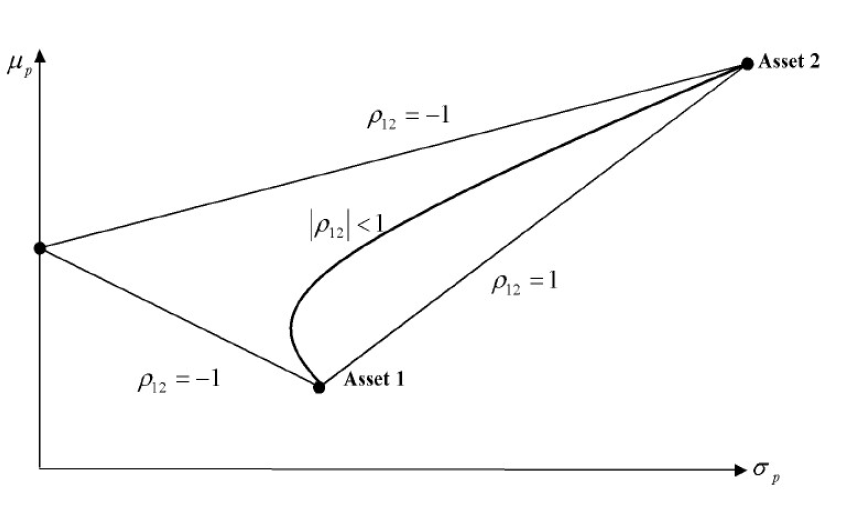
\includegraphics[width = 0.7\textwidth]{4_1.png}
\caption{$0\leq \alpha\leq 1$, when short selling is not allowed.}
\end{figure}
The feasible set will be extended by extending the corresponding line segments beyond the end points if short selling \textit{is} allowed.
\end{definition}
\subsubsection{Feasible Sets of Portfolio of Three or More Assets}
We construct the feasible sets intuitively by considering only the two-asset combination first, which gives rises to a finite set of hyperbolas and line segments. Next, we consider the combination of any two assets represented as two distinct points of these curves, which give rises to infinite number of hyperbolas and line segments. All the points on this infinite set will be inside the feasible set.

We will show that the feasible set of a portfolio with $n(>2)$ assets has the following property.
\begin{theorem}[Properties of Feasible Set]
\hfill\\\normalfont \begin{enumerate}
\item For any fixed $\mu\in\mathbb{R}$, $\exists \sigma>0$ such that $(\sigma,\mu)\in F$.
\item For each $(\sigma,\mu)\in F$, $(\sigma^\prime, \mu)\in F$ for all $\sigma^\prime>\sigma$.
\item For each pair of points $(\sigma, \mu)$ and $(\sigma^\prime, \mu^\prime)$ in the feasible set $F$, and for any $\lambda\in[0,1]$, the point $\lambda(\sigma,\mu)+(1-\lambda)(\sigma^\prime,\mu^\prime)$ lies in the set $F$. \\Equivalently, $F$ is a \textbf{convex set}.
\item For any fixed $\mu\in \mathbb{R}$, there exists $\sigma^\ast>0$ such that
\begin{enumerate}
\item $(\sigma^\ast,\mu)\in F$
\item if $(\sigma,\mu)\in F$, then $\sigma^\ast\leq \sigma$.
\end{enumerate}
We call this point $(\sigma^\ast, \mu)$ the \textbf{minimum-variance point} with mean $\mu$.
\end{enumerate}
\end{theorem}
\begin{definition}[Minimum-Variance Frontier]
\hfill\\\normalfont The theorem above suggests there is a minimum-variance point for any porfolio mean. The set of all minimum-variance points is called the \textbf{minimum-variance frontier}.
\end{definition}
It will be shown later that this minimum variance frontier is a \textbf{hyperbolic} curve.
\begin{definition}[Global Minimum Variance Point]
\hfill\\\normalfont The extreme left point on this frontier is called the \textbf{global minimum variance point}.
\end{definition}
\begin{definition}[Efficient Frontier]
\hfill\\\normalfont The minimum variance frontier \textit{above} the global minimum variance point is called the \textbf{efficient frontier}.
\end{definition}
\clearpage 
\section{Portfolio Theory \& Capital Asset Pricing Model}
\subsection{Markowitz's Portfolio Theory}
Given $n$ risky assets with mean vector $\mathbf{\mu}=\begin{pmatrix}\mu_1&\mu_2&\cdots&\mu_n\end{pmatrix}^\text{T}$ and covariance matrix $\mathbf{C}=(\rho_{ij})_{n\times n}$, we seek a portfolio $\mathbf{w}$ with the smallest portfolio risk.\\Let $\mu_p =\mathbf{w}^\text{T}\mathbf{\mu}$ denote the portfolio mean and $\sigma_p^2 = \mathbf{w}^\text{T}\mathbf{Cw}$ denote the portfolio variance.

We have two further assumptions:
\begin{enumerate}
\item[Assumption 1] $\mathbf{\mu} = \begin{pmatrix}\mu_1&\mu_2&\cdots&\mu_n\end{pmatrix}^\text{T}$ is \textit{not} a scalar multiple of $\mathbf{1}$.\footnote{If so, we have $\mu_p = \mathbf{w}^\text{T}(k\mathbf{1})=k$ a constant, which is degenerate.}
\item[Assumption 2] $\mathbf{C} = (\sigma_{ij})_{n\times n}$ is \textit{positive definite}. Equivalently, $\forall \mathbf{x}\neq \mathbf{0}, \mathbf{x}^\text{T}\mathbf{Cx}>0$.\footnote{Note $C$ as the covariance matrix is positive semidefinite. Should $\exists \mathbf{x}\neq \mathbf{0}$, such that $\mathbf{x}^\text{T}\mathbf{Cx}=0$, we can normalise $\mathbf{x}$ using 1-norm, and the left hand side become some constant times some arbitrary porfolio variance, which equals 0. This suggests the portfolio variance induced by $\mathbf{C}$ is 0 for some portfolio, which is degenerate. Therefore, we exclude the degenerate case from consideration.}
\end{enumerate}
\subsubsection{Minimisation of Portfolio Risk}
\end{document}